%%% -*- Mode: LaTeX; indent-tabs-mode: nil -*-
%%%
%%% Copyright (c) 2004, Oliver Markovic <entrox@entrox.org> 
%%%   All rights reserved. 
%%%
%%% Redistribution and use in source and binary forms, with or without
%%% modification, are permitted provided that the following conditions are met:
%%%
%%%  o Redistributions of source code must retain the above copyright notice,
%%%    this list of conditions and the following disclaimer. 
%%%  o Redistributions in binary form must reproduce the above copyright
%%%    notice, this list of conditions and the following disclaimer in the
%%%    documentation and/or other materials provided with the distribution. 
%%%  o Neither the name of the author nor the names of the contributors may be
%%%    used to endorse or promote products derived from this software without
%%%    specific prior written permission. 
%%%
%%% THIS SOFTWARE IS PROVIDED BY THE COPYRIGHT HOLDERS AND CONTRIBUTORS "AS IS"
%%% AND ANY EXPRESS OR IMPLIED WARRANTIES, INCLUDING, BUT NOT LIMITED TO, THE
%%% IMPLIED WARRANTIES OF MERCHANTABILITY AND FITNESS FOR A PARTICULAR PURPOSE
%%% ARE DISCLAIMED.  IN NO EVENT SHALL THE COPYRIGHT OWNER OR CONTRIBUTORS BE
%%% LIABLE FOR ANY DIRECT, INDIRECT, INCIDENTAL, SPECIAL, EXEMPLARY, OR
%%% CONSEQUENTIAL DAMAGES (INCLUDING, BUT NOT LIMITED TO, PROCUREMENT OF
%%% SUBSTITUTE GOODS OR SERVICES; LOSS OF USE, DATA, OR PROFITS; OR BUSINESS
%%% INTERRUPTION) HOWEVER CAUSED AND ON ANY THEORY OF LIABILITY, WHETHER IN
%%% CONTRACT, STRICT LIABILITY, OR TORT (INCLUDING NEGLIGENCE OR OTHERWISE)
%%% ARISING IN ANY WAY OUT OF THE USE OF THIS SOFTWARE, EVEN IF ADVISED OF THE
%%% POSSIBILITY OF SUCH DAMAGE.


\documentclass[a4paper]{report}

\usepackage{ngerman, graphicx, color,verbatim, hyperref}
\usepackage[T1]{fontenc}
\usepackage[latin1]{inputenc}
%\parindent 0pt
\date{\today}


\title{Entwurf MAR-S}

\begin{document}

\maketitle

\tableofcontents

% -----------------------------------------------------------------------------

%%% -*- Mode: LaTeX; indent-tabs-mode: nil -*-
%%%
%%% Copyright (c) 2004, Oliver Markovic <entrox@entrox.org> 
%%%   All rights reserved. 
%%%
%%% Redistribution and use in source and binary forms, with or without
%%% modification, are permitted provided that the following conditions are met:
%%%
%%%  o Redistributions of source code must retain the above copyright notice,
%%%    this list of conditions and the following disclaimer. 
%%%  o Redistributions in binary form must reproduce the above copyright
%%%    notice, this list of conditions and the following disclaimer in the
%%%    documentation and/or other materials provided with the distribution. 
%%%  o Neither the name of the author nor the names of the contributors may be
%%%    used to endorse or promote products derived from this software without
%%%    specific prior written permission. 
%%%
%%% THIS SOFTWARE IS PROVIDED BY THE COPYRIGHT HOLDERS AND CONTRIBUTORS "AS IS"
%%% AND ANY EXPRESS OR IMPLIED WARRANTIES, INCLUDING, BUT NOT LIMITED TO, THE
%%% IMPLIED WARRANTIES OF MERCHANTABILITY AND FITNESS FOR A PARTICULAR PURPOSE
%%% ARE DISCLAIMED.  IN NO EVENT SHALL THE COPYRIGHT OWNER OR CONTRIBUTORS BE
%%% LIABLE FOR ANY DIRECT, INDIRECT, INCIDENTAL, SPECIAL, EXEMPLARY, OR
%%% CONSEQUENTIAL DAMAGES (INCLUDING, BUT NOT LIMITED TO, PROCUREMENT OF
%%% SUBSTITUTE GOODS OR SERVICES; LOSS OF USE, DATA, OR PROFITS; OR BUSINESS
%%% INTERRUPTION) HOWEVER CAUSED AND ON ANY THEORY OF LIABILITY, WHETHER IN
%%% CONTRACT, STRICT LIABILITY, OR TORT (INCLUDING NEGLIGENCE OR OTHERWISE)
%%% ARISING IN ANY WAY OUT OF THE USE OF THIS SOFTWARE, EVEN IF ADVISED OF THE
%%% POSSIBILITY OF SUCH DAMAGE.

\chapter{Einleitung}
\section{Das Projekt Mar-S}
Das Projekt Mar-S wird durchgef�hrt, um eine Steuerung f�r den Sinnesraum am OIC zu entwickeln. 
Ziel der Software ist es in Umgebungen gleicher Ausstattung wieder verwendet zu werden.
Da immer wieder neue Komponenten hinzukommen k�nnen, mu� gew�hrleistet sein, da� diese mit minimalem Aufwand hinzugef�gt werden k�nnen. Also ohne direkt den Code zu �ndern.
In der ersten Version besteht der Sinnesraum und dessen zu entwickelnde Software aus folgenden Komponenten:
\begin{itemize}
\item PDA-Steuerung
\item Weboberfl�che f�r Einstellungen (Admin + User)
\item Konzept und Umsetzung der Datenhaltung f�r Mediadaten
\item Office Positioning System 
\item Datenbank 
\item Webserver 
\item Lichtsteuerung 
\item Windows XP MediaCenter Edition
\end{itemize} 
\section{"Uberblick "uber das Dokument}

%%% -*- Mode: LaTeX; indent-tabs-mode: nil -*-
%%%
%%% Copyright (c) 2004, Oliver Markovic <entrox@entrox.org> 
%%%   All rights reserved. 
%%%
%%% Redistribution and use in source and binary forms, with or without
%%% modification, are permitted provided that the following conditions are met:
%%%
%%%  o Redistributions of source code must retain the above copyright notice,
%%%    this list of conditions and the following disclaimer. 
%%%  o Redistributions in binary form must reproduce the above copyright
%%%    notice, this list of conditions and the following disclaimer in the
%%%    documentation and/or other materials provided with the distribution. 
%%%  o Neither the name of the author nor the names of the contributors may be
%%%    used to endorse or promote products derived from this software without
%%%    specific prior written permission. 
%%%
%%% THIS SOFTWARE IS PROVIDED BY THE COPYRIGHT HOLDERS AND CONTRIBUTORS "AS IS"
%%% AND ANY EXPRESS OR IMPLIED WARRANTIES, INCLUDING, BUT NOT LIMITED TO, THE
%%% IMPLIED WARRANTIES OF MERCHANTABILITY AND FITNESS FOR A PARTICULAR PURPOSE
%%% ARE DISCLAIMED.  IN NO EVENT SHALL THE COPYRIGHT OWNER OR CONTRIBUTORS BE
%%% LIABLE FOR ANY DIRECT, INDIRECT, INCIDENTAL, SPECIAL, EXEMPLARY, OR
%%% CONSEQUENTIAL DAMAGES (INCLUDING, BUT NOT LIMITED TO, PROCUREMENT OF
%%% SUBSTITUTE GOODS OR SERVICES; LOSS OF USE, DATA, OR PROFITS; OR BUSINESS
%%% INTERRUPTION) HOWEVER CAUSED AND ON ANY THEORY OF LIABILITY, WHETHER IN
%%% CONTRACT, STRICT LIABILITY, OR TORT (INCLUDING NEGLIGENCE OR OTHERWISE)
%%% ARISING IN ANY WAY OUT OF THE USE OF THIS SOFTWARE, EVEN IF ADVISED OF THE
%%% POSSIBILITY OF SUCH DAMAGE.

\chapter{System}

\section{Verwendete Technologien}
Folgende Technologien werden verwendet:
\begin{itemize}
\item Eclipse 3.0.2 (Entwicklungumgebung f�r Java)
\item Hiberclipse 2.0.1 (Hibernate-Plugin f�r Eclipse)
\item Hibernate (Datenbank-Mapping Framework)
\item PostgreSQL 8.0 (Datenbanksystem des Mar-S-Systems)
\item Apache Tomcat 5.5.9 (Server)
\item Jakarta Struts 1.2.7 (Webapplication Framework)
\item JDK 5.0 (Java VM und SDK)
\item C\# 
\item Windows XP Media Center Edition 2005
\item C++
\end{itemize}

%%% -*- Mode: LaTeX; indent-tabs-mode: nil -*-
%%%
%%% Copyright (c) 2004, Oliver Markovic <entrox@entrox.org> 
%%%   All rights reserved. 
%%%
%%% Redistribution and use in source and binary forms, with or without
%%% modification, are permitted provided that the following conditions are met:
%%%
%%%  o Redistributions of source code must retain the above copyright notice,
%%%    this list of conditions and the following disclaimer. 
%%%  o Redistributions in binary form must reproduce the above copyright
%%%    notice, this list of conditions and the following disclaimer in the
%%%    documentation and/or other materials provided with the distribution. 
%%%  o Neither the name of the author nor the names of the contributors may be
%%%    used to endorse or promote products derived from this software without
%%%    specific prior written permission. 
%%%
%%% THIS SOFTWARE IS PROVIDED BY THE COPYRIGHT HOLDERS AND CONTRIBUTORS "AS IS"
%%% AND ANY EXPRESS OR IMPLIED WARRANTIES, INCLUDING, BUT NOT LIMITED TO, THE
%%% IMPLIED WARRANTIES OF MERCHANTABILITY AND FITNESS FOR A PARTICULAR PURPOSE
%%% ARE DISCLAIMED.  IN NO EVENT SHALL THE COPYRIGHT OWNER OR CONTRIBUTORS BE
%%% LIABLE FOR ANY DIRECT, INDIRECT, INCIDENTAL, SPECIAL, EXEMPLARY, OR
%%% CONSEQUENTIAL DAMAGES (INCLUDING, BUT NOT LIMITED TO, PROCUREMENT OF
%%% SUBSTITUTE GOODS OR SERVICES; LOSS OF USE, DATA, OR PROFITS; OR BUSINESS
%%% INTERRUPTION) HOWEVER CAUSED AND ON ANY THEORY OF LIABILITY, WHETHER IN
%%% CONTRACT, STRICT LIABILITY, OR TORT (INCLUDING NEGLIGENCE OR OTHERWISE)
%%% ARISING IN ANY WAY OUT OF THE USE OF THIS SOFTWARE, EVEN IF ADVISED OF THE
%%% POSSIBILITY OF SUCH DAMAGE.

\chapter{Controller}

\section{Generelles Konzept zur Businesslogik}

\begin{figure}[!h]
\begin{center}
  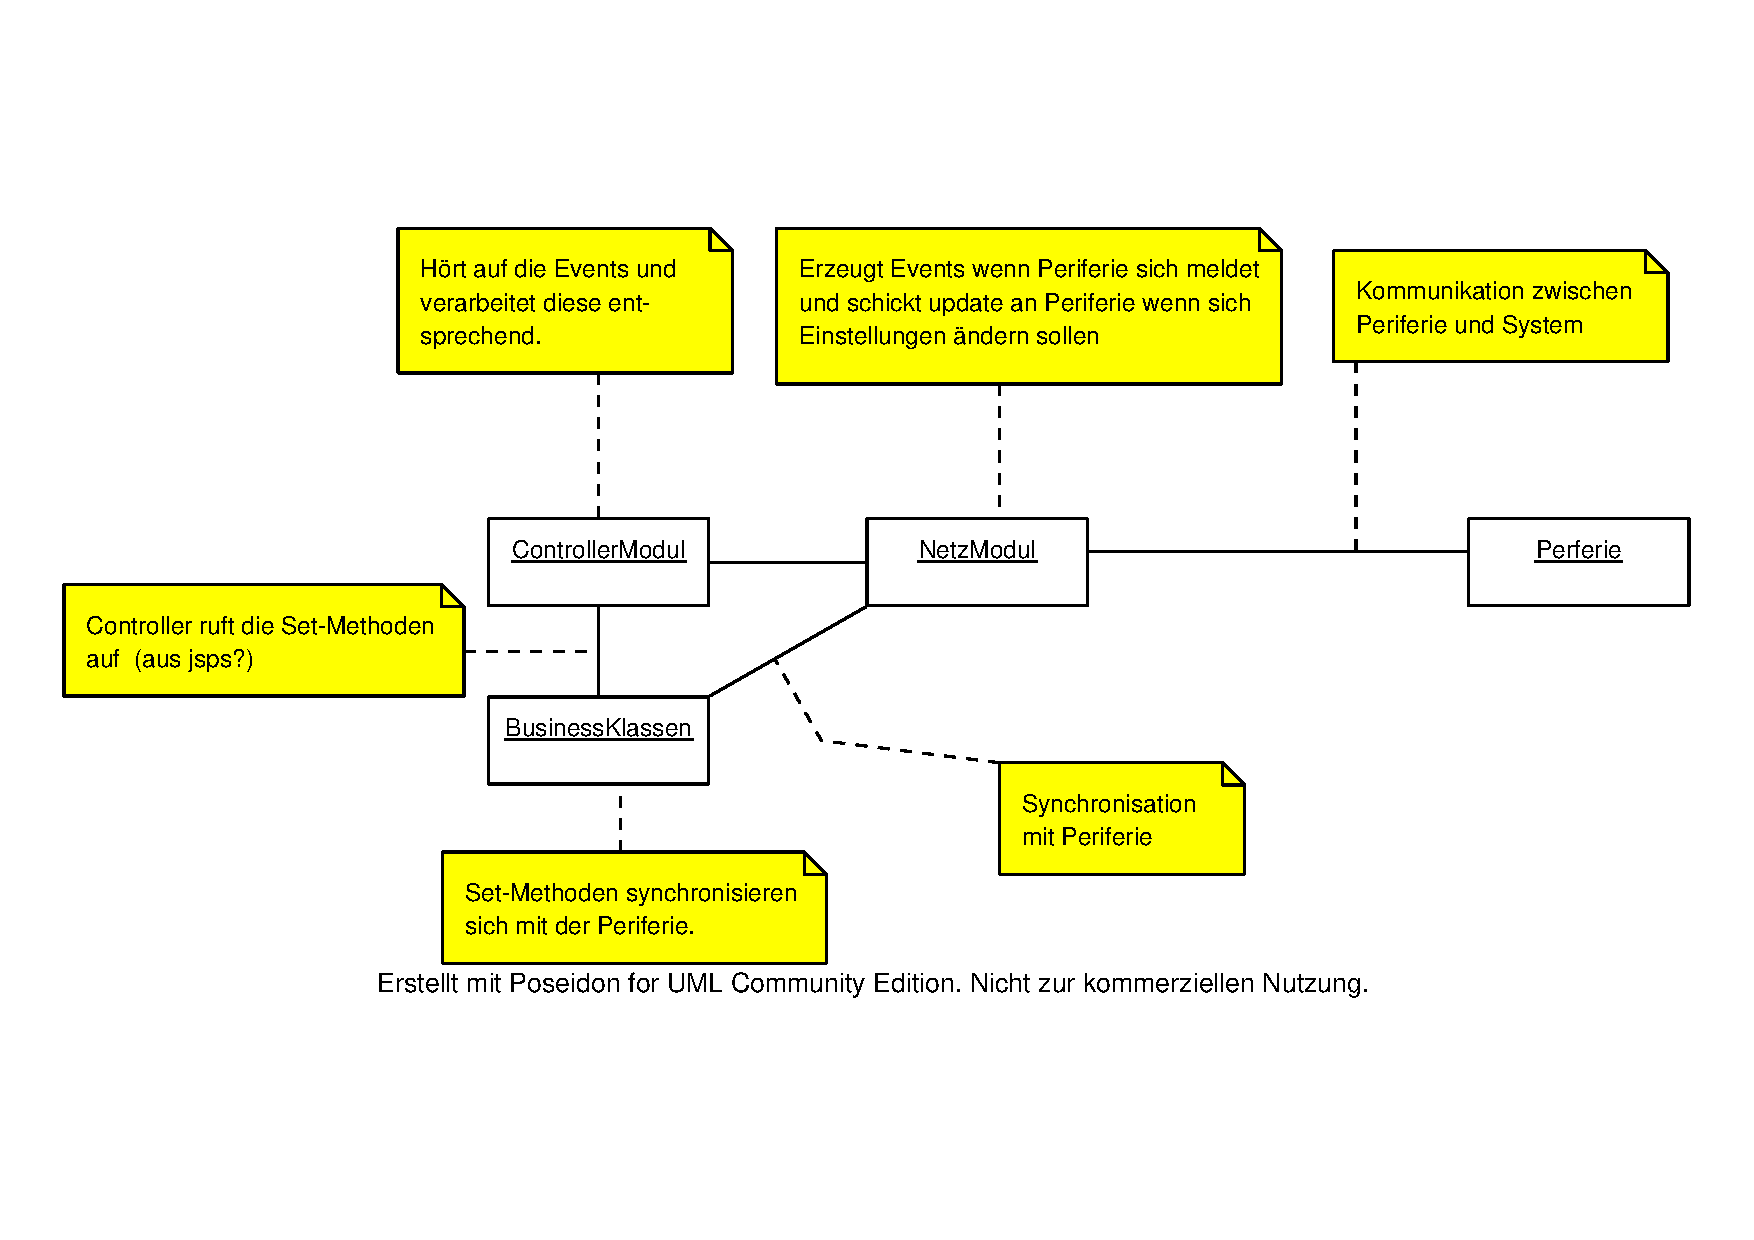
\includegraphics[width=360pt]{logischer_zusammenhang_controller.pdf}
  \caption{Zusammenhang der Komponenten}
\end{center}
\vspace*{-6mm}
\end{figure}
\newpage
\section{Beschreibung der Logik}
Im Folgenden wird der Entwurf der grundlegenden Szenarien beschrieben.\\
\begin{itemize}
\item Szenario 1: Das System wird gestartet.
\item Szenario 2: Ein Benutzer betritt den Raum.
\item Szenario 3: Ein Benutzer �ndert seine Profileinstellungen.
\end{itemize}

\subsection{Klassen und Methodenbeschreibung}

\begin{figure}[!h]
\begin{center}
  \includegraphics[width=360pt]{Klassen_Controller.pdf}
  \caption{Klassen und Methoden f�r die Businesslogic}
\end{center}
\vspace*{-6mm}
\end{figure}

\subsubsection{BusinessKlassen}

\textbf{UserLogin logIn()}
\begin{itemize}
	\item Meldet den Benutzer am Betriebsystem an.
	\item Setzt den Benutzer auf eingeloggt.
	\item L�dt das Defaultprofil des Benutzers\\
\end{itemize}

\textbf{UserLogin logOut()}
\begin{itemize}
	\item Meldet den Benutzer vom Betriebsystem ab.
	\item Setzt den Benutzer auf nicht eingeloggt.
	\item Setzt alle Komponenten auf ihre Defaulteinstellung.\\
\end{itemize}

\textbf{SmartRoomComponent static getComponent(String description)}
Der Wert \textit{description} enth�llt die id der Komponente.
\begin{itemize}
	\item Falls die Komponenten-Instanz mit der id schon existiert (im Speicher), liefert sie zur�ck.
	\item Falls die Komponenten-Instanz mit der id noch nicht existiert, wird die Komponenten-Instanz anhand der description erzeugt.\\
\end{itemize}

\textbf{SmartRoomComponent remove()}
\begin{itemize}
	\item Entfernt alle Eintr�ge aus den Benutzerprofilen, die zu dieser Komponente geh�ren .\\
\end{itemize}

\textbf{SmartRoomComponent setIsActive(Boolean isActive)}
\begin{itemize}
	\item Setzt die Komponenten-Instanz auf aktiv / inaktiv.
	\item Nur aktive Komponenten werden angezeigt.\\
\end{itemize}

\textbf{SmartRoomProfil load()}
\begin{itemize}
	\item Setzt alle zum Profil geh�rigen Properties. 
	\item Das Setzen der Properties bewirkt deren synchronisation mit der Periferie.\\
\end{itemize}

\textbf{ComponentProperie setValue(ComponentProperieValue value)}
\begin{itemize}
	\item Wenn Benutzer eingeloggt ist, Synchronisation mit der Periferie.\\
\end{itemize}


\textbf{NetzContoller StandardEvents}
\begin{itemize}
	\item signalUserIn (OPS) - Ein Benutzer hat den Raum betreten. 
	\item signalUserOut (OPS) - Ein Benutzer hat den Raum verlassen. 
	\item signalPropertieChange (MediaCenter) - Eine Properie wurde gesetzt/ver�ndert.\\
\end{itemize}

\textbf{NetzContoller init()}
\begin{itemize}
	\item sendet broadcast, woraufhin sich alle Componenten melden sollen.\\
\end{itemize}

\textbf{NetzContoller signal(Event event)}
\begin{itemize}
	\item l�st ein Event aus.\\
\end{itemize}


\textbf{UserEventListener handleEvent()}
\begin{tabbing}
xxxx\=xxxxxxxxx \kill
Auf: "`TagID rein"'\\
\>-> Hohl Benutzer; Benutzer.logIn();\\
Auf: "`Benutzer rein"'\\
\>-> Benutzer.logIn();\\
Auf: "`Benutzer raus"'\\
\>-> Benutzer.logOut();\\
Auf "`TagID raus"'\\
\>-> Hohl Benutzer; Benutzer.logOut();\\
\end{tabbing}


\textbf{MarsComponentListener initComponents()}
\begin{itemize}
	\item Initialisiert das Netz\\
\end{itemize}

\textbf{MarsComponentListener handleEvent()}
\begin{tabbing}
xxxx\=xxx\=xxxxxx \kill
1. Auf: "`Hallo, ich bin da"'\\
		\>-> ist Componente schon initialisiert und ist sie aktuell.\\
    \>\> true -> nix\\
    \>\> false -> hohle Beschreibung; initialisiere Componente mit Beschreibung;\\
2. Auf: "`Tsch�ss"'\\
    \>-> ist Componente bekannt:\\
    \>\> true -> Componente.setIsActive(false);\\
\end{tabbing}

\textbf{MarsComponentListener setProperie(String id, PropertyValue value)}
\begin{itemize}
	\item L�dt Property mit dazugeh�riger ID
	\item Setzt das Value der Propery mit Value
\end{itemize}

\subsection{Szenario 1 - Starten des Systems}
Das Netzmodul sendet einen Broadcast ins Netz, woraufhin sich die einzelnen Komponenten melden.
Das Netzmodul signalisiert jede sich meldende Komponente an den Komponenten-Listener. Dieser speichert die Beschreibungen zur Komponente in der Datenbank.

\subsection{Szenario 1 - Ein Benutzer betritt der Raum}
Das OPS signalisiert "`BenutzerX hat den Raum betreten"'. Der UserController meldet den Benutzer am Betriebsystem an und l�dt dessen Defaultprofil.

\subsection{Szenario 3: Ein Benutzer �ndert seine Profileinstellungen.}
Ein Benutzer �ndert �ber das MediaCenter seine Einstellungen. Das MediaCenter signalisiert: PropertyX hat sich auf ValueX ge�ndert. Der ComponentenListener setzt die entsprechende Property im Speicher auf das gegebene Value. Durch den Setzvorgang wird die Periferie synchronisiert.

\chapter{Logon Logik}
\section{Logon-Szenarien}
Der Logon f�r das System des Sinnesraumes kann �ber zwei Arten erfolgen. Die erste Art ist,
 da� ein Tag durch das OPS innerhalb des Raumes erkannt wurde. Hierf�r meldet das OPS dem Controller alle Tags die den Raum betreten und wieder verlassen. Die zweite M�glichkeit ist der manuelle Logon �ber ein PDA (Eingabe von Benutzernamen und Passwort).
\\
Da immer nur ein Benutzer eingeloggt sein kann, wurde folgendes Rechtekonzept entwickelt, 
um die Logonvarianten zu regeln.

\begin{figure}[!h]
\begin{center}
  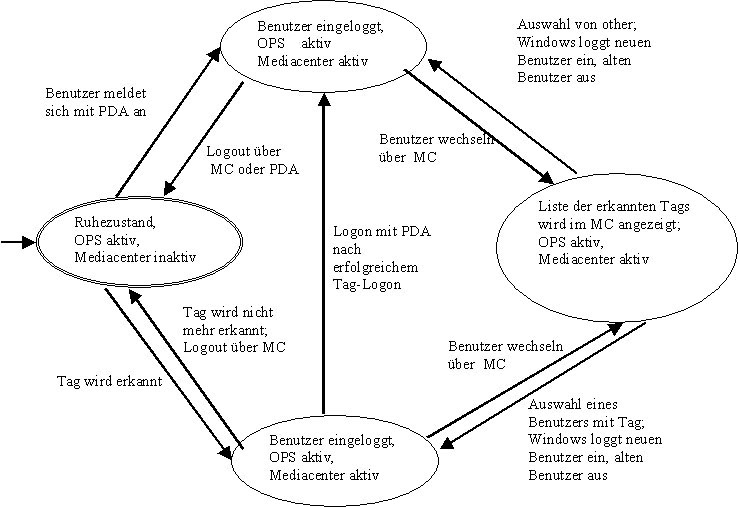
\includegraphics[width=360pt]{positioning.jpg}
  \caption{�bersicht Logon-Szenarien}
\end{center}
\vspace*{-6mm}
\end{figure}

\subsection{Logon aus dem Ruhezustand des Systems (Tagbasiert)}
\subsubsection*{Ausgangssituation}
\begin{itemize}
\item System: Ruhezustand
\item OPS: aktiv
\item Mediacenter: inaktiv
\end{itemize}
\subsubsection*{Logonvorgang}
Der Benutzer, dessen Tag-Id zuerst an den Controller geschickt wird,
wird vom System eingeloggt. Hierzu wird �ber den Controller an das Betriebssystem eine
Nachricht geschickt.
\subsubsection*{Erreichte Situation}
\begin{itemize}
\item System: User eingeloggt (tagbasiert)
\item OPS: aktiv
\item Mediacenter: aktiv
\end{itemize}


\subsection{Logon aus dem Ruhezustand des Systems (PDA-basiert)}
\subsubsection*{Ausgangssituation}
\begin{itemize}
\item System: Ruhezustand
\item OPS: aktiv
\item Mediacenter: inaktiv
\end{itemize}
\subsubsection*{Logonvorgang}
Der Benutzer baut eine Verbindung zwischen seinem PDA und dem Rechner im Sinnesraum auf.\\
Auf der Weboberfl�che seines PDAs kann der Benutzer seinen User-Namen und sein Passwort eingeben.
Dieser wird mit den Daten in der Datenbank �berpr�ft und bei �bereinstimmung der Daten wird der Benutzer 
vom System eingeloggt. Hierzu wird �ber den Controller an das Betriebssystem eine
Nachricht geschickt.\\
Dieser Logonvorgang wird beispielsweise ben�tigt, sollte ein Benutzer sein Tag nicht dabei haben.
\subsubsection*{Erreichte Situation}
\begin{itemize}
\item System: User eingeloggt (PDA-basiert)
\item OPS: aktiv
\item Mediacenter: aktiv
\end{itemize}

\subsection{Change User (Tag-eingeloggt) zu einem anderen Benutzer mit Tag}
\subsubsection*{Ausgangssituation}
\begin{itemize}
\item System: User eingeloggt (tagbasiert)
\item OPS: aktiv 
\item Mediacenter: aktiv
\end{itemize}
\subsubsection*{Logonvorgang}
Der Benutzer hat die M�glichkeit sich �ber das Mediacenter alle Tags, die sich im Raum befinden,  
anzeigen zu lassen. Durch Anklicken des jeweiligen Benutzernamens wird der alte User aus- und der 
ausgew�hlte User eingeloggt.
\subsubsection*{Erreichte Situation}
\begin{itemize}
\item System: User eingeloggt (tagbasiert)
\item OPS: aktiv
\item Mediacenter: aktiv
\end{itemize}

\subsection{Change User (PDA-eingeloggt) zu einem anderen Benutzer mit Tag}
\subsubsection*{Ausgangssituation}
\begin{itemize}
\item System: User eingeloggt (tagbasiert)
\item OPS: aktiv 
\item Mediacenter: aktiv
\end{itemize}
\subsubsection*{Logonvorgang}
Der Benutzer hat die M�glichkeit sich �ber das Mediacenter alle Tags, die sich im Raum befinden,  
anzeigen zu lassen. Durch Anklicken des jeweiligen Benutzernamens wird der alte User aus- und der ausgew�hlte User eingeloggt.
\subsubsection*{Erreichte Situation}
\begin{itemize}
\item System: User eingeloggt (tagbasiert)
\item OPS: aktiv
\item Mediacenter: aktiv
\end{itemize}

\subsection{Change User (Tag-eingeloggt) zu einem anderen Benutzer mit PDA}
\subsubsection*{Ausgangssituation}
\begin{itemize}
\item System: User eingeloggt (tagbasiert)
\item OPS: aktiv 
\item Mediacenter: aktiv
\end{itemize}
\subsubsection*{Logonvorgang}
Der Benutzer hat die M�glichkeit sich �ber das Mediacenter alle Tags, die sich im Raum befinden,  
anzeigen zu lassen. Durch Anklicken von other kann sich mit dem PDA einloggen.
\subsubsection*{Erreichte Situation}
\begin{itemize}
\item System: User eingeloggt (PDA-basiert)
\item OPS: aktiv
\item Mediacenter: aktiv
\end{itemize}

\subsection{Change User (PDA-eingeloggt) zu einem anderen Benutzer mit PDA}
\subsubsection*{Ausgangssituation}
\begin{itemize}
\item System: User eingeloggt (tagbasiert)
\item OPS: aktiv 
\item Mediacenter: aktiv
\end{itemize}
\subsubsection*{Logonvorgang}
Der Benutzer hat die M�glichkeit sich �ber das Mediacenter alle Tags, die sich im Raum befinden,  
anzeigen zu lassen.Durch Anklicken von other kann sich mit dem PDA einloggen. 
\subsubsection*{Erreichte Situation}
\begin{itemize}
\item System: User eingeloggt (PDA-basiert)
\item OPS: aktiv
\item Mediacenter: aktiv
\end{itemize}

\subsection{Logon mit PDA nach erfolgreichem Tag-Logon}
Will ein Benutzer nicht mit dem Trackball navigieren, sondern mit seinem PDA, so kann er sich einfach mit dem PDA einloggen.
\subsubsection*{Ausgangssituation}
\begin{itemize}
\item System: User eingeloggt (tagbasiert)
\item OPS: aktiv 
\item Mediacenter: aktiv
\end{itemize}
\subsubsection*{Logonvorgang}
Der Benutzer verbindet sich mit seinem PDA zum Rechner und gibt sein Benutzernamen
 und sein Passwort ein. Die Daten werden mit denen des eingeloggten Users verglichen.
 Sollte es der identische User sein, so wird er PDA-basiert eingeloggt. Das laufende 
 Programm wird nicht unterbrochen. Sollte es sich um einen anderen User handeln, passiert nichts.
\subsubsection*{Erreichte Situation}
\begin{itemize}
\item System: User eingeloggt (PDA-basiert)
\item OPS: aktiv
\item Mediacenter: aktiv
\end{itemize}

\section{Logoutszenarien}
\subsection{Automatisches Logout eines tagbasierten Users}
\subsubsection*{Ausgangssituation}
\begin{itemize}
\item System: User eingeloggt (tagbasiert)
\item OPS: aktiv 
\item Mediacenter: aktiv
\end{itemize}
\subsubsection*{Logoutvorgang}
Wird das Signal eines tagbasierten Users nicht mehr erkannt, 
so wird dieser automatisch ausgeloggt.
\subsubsection*{Erreichte Situation}
\begin{itemize}
\item System: Ruhezustand
\item OPS: aktiv
\item Mediacenter: inaktiv
\end{itemize}

\subsection{Manuelles Logout eines tagbasierten Users}
\subsubsection*{Ausgangssituation}
\begin{itemize}
\item System: User eingeloggt (tagbasiert)
\item OPS: aktiv 
\item Mediacenter: aktiv
\end{itemize}
\subsubsection*{Logonvorgang}
Ein User kann �ber logout im MediaCenter jeden anderen Benutzer ausloggen. \\
Der User der zuletzt eingeloggt war, kann f�r 30 Sekunden nicht �ber seinen Tag eingeloggt werden.
\subsubsection*{Erreichte Situation}
\begin{itemize}
\item System: Ruhezustand
\item OPS: aktiv
\item Mediacenter: inaktiv
\end{itemize}

\subsection{Logout eines PDA-basierten Users}
\subsubsection*{Ausgangssituation}
\begin{itemize}
\item System: User eingeloggt (PDA-basiert)
\item OPS: inaktiv 
\item Mediacenter: aktiv
\end{itemize}
\subsubsection*{Logonvorgang}
Ein User kann �ber logout im MediaCenter jeden anderen Benutzer ausloggen. Der User kann sich aber auch selbst �ber sein PDA ausloggen.\\
Der User der zuletzt eingeloggt war, kann f�r 30 Sekunden nicht �ber seinen Tag eingeloggt werden.
\subsubsection*{Erreichte Situation}
\begin{itemize}
\item System: Ruhezustand
\item OPS: aktiv
\item Mediacenter: inaktiv
\end{itemize}

%%% -*- Mode: LaTeX; indent-tabs-mode: nil -*-
%%%
%%% Copyright (c) 2004, Oliver Markovic <entrox@entrox.org> 
%%%   All rights reserved. 
%%%
%%% Redistribution and use in source and binary forms, with or without
%%% modification, are permitted provided that the following conditions are met:
%%%
%%%  o Redistributions of source code must retain the above copyright notice,
%%%    this list of conditions and the following disclaimer. 
%%%  o Redistributions in binary form must reproduce the above copyright
%%%    notice, this list of conditions and the following disclaimer in the
%%%    documentation and/or other materials provided with the distribution. 
%%%  o Neither the name of the author nor the names of the contributors may be
%%%    used to endorse or promote products derived from this software without
%%%    specific prior written permission. 
%%%
%%% THIS SOFTWARE IS PROVIDED BY THE COPYRIGHT HOLDERS AND CONTRIBUTORS "AS IS"
%%% AND ANY EXPRESS OR IMPLIED WARRANTIES, INCLUDING, BUT NOT LIMITED TO, THE
%%% IMPLIED WARRANTIES OF MERCHANTABILITY AND FITNESS FOR A PARTICULAR PURPOSE
%%% ARE DISCLAIMED.  IN NO EVENT SHALL THE COPYRIGHT OWNER OR CONTRIBUTORS BE
%%% LIABLE FOR ANY DIRECT, INDIRECT, INCIDENTAL, SPECIAL, EXEMPLARY, OR
%%% CONSEQUENTIAL DAMAGES (INCLUDING, BUT NOT LIMITED TO, PROCUREMENT OF
%%% SUBSTITUTE GOODS OR SERVICES; LOSS OF USE, DATA, OR PROFITS; OR BUSINESS
%%% INTERRUPTION) HOWEVER CAUSED AND ON ANY THEORY OF LIABILITY, WHETHER IN
%%% CONTRACT, STRICT LIABILITY, OR TORT (INCLUDING NEGLIGENCE OR OTHERWISE)
%%% ARISING IN ANY WAY OUT OF THE USE OF THIS SOFTWARE, EVEN IF ADVISED OF THE
%%% POSSIBILITY OF SUCH DAMAGE.

\chapter{OPS}
\section{Einleitung}
Im Sinnesraum gibt es generell zwei M�glichkeiten sich am System anzumelden. 
Die eine Variante ist die tagbasierte, die andere die PDA-basierte.
Bei beiden Varianten hat der Benutzer das System zu steuern. Wie der Login-Prozess 
genau auf Betriebssystemebene abl�uft, ist im Kapitel Betriebssystem nachzulesen.\\
Um ein Benutzer tagbasiert einloggen zu k�nnen, mu� das System wissen, wer sich im Raum befindet.
\section{Tag-Logik}
Die einzelnen Benutzer verf�gen �ber Tags, welche alle 1,5 Sekunden ein Signal an die Empfangsantenne schicken.
\\
Wird nun ein Benutzer zweimal innerhalb von 6 Sekunden erkannt so wird er als im Raum befindlich gesehen.\\
Ist dies nicht der Fall, so wird er nicht als im Raum befindlich gesehen. Die Komponente OPS schickt also alle sechs Sekunden eine Nachricht an den Controller, ob eine Person den Raum verlassen oder betreten hat.
\section{Klassen}
Die Komponente OPS besteht quasi aus 3 Klassen.
\begin{itemize}
\item Eine Klasse stellt eine Verbindung zu einer seriellen Schnittstelle her.
\item Eine Klasse erh�lt die Nachrichten von der seriellen Schnitstelle.
\item Eine Klasse enth�lt die Logik, ob sich ein Benutzer im Raum befindet oder nicht.
\end{itemize}





%%% -*- Mode: LaTeX; indent-tabs-mode: nil -*-
%%%
%%% Copyright (c) 2004, Oliver Markovic <entrox@entrox.org> 
%%%   All rights reserved. 
%%%
%%% Redistribution and use in source and binary forms, with or without
%%% modification, are permitted provided that the following conditions are met:
%%%
%%%  o Redistributions of source code must retain the above copyright notice,
%%%    this list of conditions and the following disclaimer. 
%%%  o Redistributions in binary form must reproduce the above copyright
%%%    notice, this list of conditions and the following disclaimer in the
%%%    documentation and/or other materials provided with the distribution. 
%%%  o Neither the name of the author nor the names of the contributors may be
%%%    used to endorse or promote products derived from this software without
%%%    specific prior written permission. 
%%%
%%% THIS SOFTWARE IS PROVIDED BY THE COPYRIGHT HOLDERS AND CONTRIBUTORS "AS IS"
%%% AND ANY EXPRESS OR IMPLIED WARRANTIES, INCLUDING, BUT NOT LIMITED TO, THE
%%% IMPLIED WARRANTIES OF MERCHANTABILITY AND FITNESS FOR A PARTICULAR PURPOSE
%%% ARE DISCLAIMED.  IN NO EVENT SHALL THE COPYRIGHT OWNER OR CONTRIBUTORS BE
%%% LIABLE FOR ANY DIRECT, INDIRECT, INCIDENTAL, SPECIAL, EXEMPLARY, OR
%%% CONSEQUENTIAL DAMAGES (INCLUDING, BUT NOT LIMITED TO, PROCUREMENT OF
%%% SUBSTITUTE GOODS OR SERVICES; LOSS OF USE, DATA, OR PROFITS; OR BUSINESS
%%% INTERRUPTION) HOWEVER CAUSED AND ON ANY THEORY OF LIABILITY, WHETHER IN
%%% CONTRACT, STRICT LIABILITY, OR TORT (INCLUDING NEGLIGENCE OR OTHERWISE)
%%% ARISING IN ANY WAY OUT OF THE USE OF THIS SOFTWARE, EVEN IF ADVISED OF THE
%%% POSSIBILITY OF SUCH DAMAGE.

\chapter{Datenschicht}
\section{Allgemein}
Im folgenden wir das Datenmodell des Mar-s Systems beschrieben. Die Beschreibung orientiert sich am UML-Klassendiagramm des zu entwerfenden Systems. Das Datenbankschema wird nicht weiter beschrieben, da es aus dem Datenmodell (Klassendiagramm) generiert wird. Das Mapping zwischen den Datenklassen des Klassendiagramms und den Datenbanktabellen �bernimmt das Mappingframework \textbf{HIBERNATE}. 
\newpage

\section{Datenmodell/Klassendiagramm}
Aus Gr�nden der �bersichtlichkeit sind die Methoden der Klassen im nachfolgenden Diagramm ausgeblendet. 
\begin{figure}[!h]
\begin{center}
  \includegraphics[width=360pt]{Klassendiagramm.png}
  \caption{Klassendiagramm}
\end{center}
\vspace*{-6mm}
\end{figure}


\section{Beschreibung der Datenklassen}

\subsection{Klasse: \textit{Department}}
Enth�lt Informationen zu den Abteilungen in der Einsatzumgebung des Mar-s Systems. Dient der Verwaltung der User. Verwaltet werden Abt.-name, -k�rzel und ein Kommentarfeld. 

\subsection{Klasse: \textit{User}}
Speichert alle Benutzers die im Mar-S System registriert sind. 
Au�erdem beinhaltet sie alle wichtigen Daten um die Anmeldung am Betriebssystem (MS Windows XP Mediacenter Edition), 
die Zuordnung zwischen Identifications (Anmeldungen an den SmartRoom) und Mar-s-User sowie dem Autostart von Profilen zu realisieren. Zus�tzlich ist die Quota des Users in dieser Klasse hinterlegt. Das Passwort wird aus Sicherheitsgr�nden in verschl�sselter Form in der Datenbank gespeichert (Symmetrisches Verschl�sselungsverfahren), eine Entschl�sselung muss Betriebssystembedingt (vgl. Windows-API Systemlogin) gew�hrleistet werden. �ber die Klasse \textit{User} ist der direkte Zugriff auf SmartRoomProfile m�glich.
  

\subsection{Klasse: \textit{Group}}
Diese Klassen beschreibt die Gruppen mit einem eindeutigen Name und einem Kommentarfeld. Die Gruppen verf�gen �ber ein Haltbarkeitsdatum. Wird es �berschritten wird die Gruppe sowie aller Referenzen zu ihr gel�scht.
Benutzer des Mar-s Systems k�nnen SmartRoomProfile definieren die f�r alle Mitlieder einer bestimmten Gruppe sichtbar sind. Jedes Objekt der Klasse \textit{UserLogin} geh�rt mindestens der Gruppe \underline{\textit{Public}} an.

\subsection{Klasse: \textit{LogInSystem}}
Diese Klasse repr�sentiert LogInSysteme mit denen sich ein Benutzer an den SmartRoom anmelden kann. Ein LogInSystem ist das OPS ein anderes der PDA

\subsection{Klasse: \textit{Identification}}
Identifications bestehen aus einem LogInSystem und einem f�r das LogInSystem eindeutige tagID. Jeder Benutzer kann mehrere Identifications haben.



\subsection{Klasse: \textit{SmartRoomComponent}}
Die Klasse repr�sentiert eine Komponente im SmartRoom. Eine Komponente kann mehrere Attribute (ComponenentAttributes) besitzen.

\subsection{Klasse: \textit{ComponentAttribute}}
Die Klasse beschreibt die Attribute einer Komponente bzw. die Subattribute eines �bergeordneten Attributs.
Jedes Komponentenattribut besitzt einen Wert (Siehe klasse \textit{ComponentAttributeValue}). Die �nderbarkeit der Attributwerte kann �ber das Feld editable eingeschr�nkt werden, dies ist wichtig f�r die Generierung der JSP-Seiten um Komponentenattributwerte zu modifizieren (Z.B. Lichtintensit�t) oder nur darzustellen (z.B. maximale Lichtintensit�t). Jedes Attribut hat einen bestimmten Typ (AttributeType).

\subsection{Klasse: \textit{AttributeType}}
Die Subklassen von AttributeType legen die Typen eines Attributs fest. Bisher kann ein Attribut mit Werten vom Typ String, Numeric, Boolean und List bef�llt sein. Im Attributtyp ist auch der Default-Wert f�r das Attribut fest gelegt.

\subsection{Klasse: \textit{SmartRoomProfil}}
Diese Klasse enth�lt die Raumprofile f�r den Smartroom, diese beinhalten alle Komponenten des Smartrooms. Diese Klasse erm�glicht den Zugriff auf die einzelnen Komponenten. Ein Profil besteht also aus lauter Einstellungen von Componenteneigenschaften. Diese werden in ComponentSettings zusammengefasst.

\subsection{Klasse: \textit{ComponentSetting}}
ComponentSettings fassen die konkreten Einstellungen eines Profils (SmartRoomProfile) f�r eine Komponente (SmartRoomComponent) zusammen.


\subsection{Klasse: \textit{ComponentAttributeValue}}
Instanzen dieser Klasse realisieren die Werte die das verkn�pfte ComponentAttribute annehmen soll. Wie die AttributTypen k�nnen die Values auch vom Typ Numeric, String, Boolean und List sein.

%%% -*- Mode: LaTeX; indent-tabs-mode: nil -*-
%%%
%%% Copyright (c) 2004, Oliver Markovic <entrox@entrox.org> 
%%%   All rights reserved. 
%%%
%%% Redistribution and use in source and binary forms, with or without
%%% modification, are permitted provided that the following conditions are met:
%%%
%%%  o Redistributions of source code must retain the above copyright notice,
%%%    this list of conditions and the following disclaimer. 
%%%  o Redistributions in binary form must reproduce the above copyright
%%%    notice, this list of conditions and the following disclaimer in the
%%%    documentation and/or other materials provided with the distribution. 
%%%  o Neither the name of the author nor the names of the contributors may be
%%%    used to endorse or promote products derived from this software without
%%%    specific prior written permission. 
%%%
%%% THIS SOFTWARE IS PROVIDED BY THE COPYRIGHT HOLDERS AND CONTRIBUTORS "AS IS"
%%% AND ANY EXPRESS OR IMPLIED WARRANTIES, INCLUDING, BUT NOT LIMITED TO, THE
%%% IMPLIED WARRANTIES OF MERCHANTABILITY AND FITNESS FOR A PARTICULAR PURPOSE
%%% ARE DISCLAIMED.  IN NO EVENT SHALL THE COPYRIGHT OWNER OR CONTRIBUTORS BE
%%% LIABLE FOR ANY DIRECT, INDIRECT, INCIDENTAL, SPECIAL, EXEMPLARY, OR
%%% CONSEQUENTIAL DAMAGES (INCLUDING, BUT NOT LIMITED TO, PROCUREMENT OF
%%% SUBSTITUTE GOODS OR SERVICES; LOSS OF USE, DATA, OR PROFITS; OR BUSINESS
%%% INTERRUPTION) HOWEVER CAUSED AND ON ANY THEORY OF LIABILITY, WHETHER IN
%%% CONTRACT, STRICT LIABILITY, OR TORT (INCLUDING NEGLIGENCE OR OTHERWISE)
%%% ARISING IN ANY WAY OUT OF THE USE OF THIS SOFTWARE, EVEN IF ADVISED OF THE
%%% POSSIBILITY OF SUCH DAMAGE.

\chapter{WebApp}
	
	\section{Webserver}
		\subsection{Container und Ordnerstrucktur}
			Der Webserver besteht aus einem Tomcat 5.0.x welcher als JSP Container dient. Hierdurch ergibt sich 
			auch folgende Ordnerstrucktur: 
			
				\begin{verbatim}
					...\Tomcat\webapps\mars
					...\Tomcat\webapps\mars\web
					...\Tomcat\webapps\mars\web\images
					...\Tomcat\webapps\mars\web\jsp
					...\Tomcat\webapps\mars\web\mldocs
					...\Tomcat\webapps\mars\WEB-INF
					...\Tomcat\webapps\mars\WEB-INF\classes
					...\Tomcat\webapps\mars\WEB-INF\etc
					...\Tomcat\webapps\mars\WEB-INF\etc\docs
					...\Tomcat\webapps\mars\WEB-INF\lib
					...\Tomcat\webapps\mars\WEB-INF\src
				\end{verbatim}
  		Der Standard Port des Servers ist \verb|8080| %wir baruchen da wohl noch ne IP bzw nen Hostnamen?%
  		 
		\subsection{Aufbau}
		
			\begin{center}
		 		\includegraphics[width=0.50\textwidth]{Level1.jpg}
			\end{center}
			
			Wie die Abbildung zeigt stellt sie die Anwendung dem Benutzer als eine reine html Anwendung dar. 
			An dieser Stelle wird darauf hingewiesen, dass der Einstieg in das System �ber die Seite \verb|index.html|
			erfolgt. Diese besteht aus reinem html und verweist auf die folgenden jsp Seiten.
			Dies dient dem "`Information hiding"'.
			Da es sich nicht um eine WWW Applikation handelt, wird davon abgesehen den \verb|web|-Baum unter \verb|WEB-INF|
			unterzubringen.
			    
			Die durch den User gestellten Anfragen an das System(\textit{Request})(wie z.B. nach dem Ausf"ullen eins Formulars)
			behandelt die Anwendung in Form eines Model 1\footnote{\url{http://en.wikipedia.org/wiki/Model_2}} (siehe Abbildung).
			
			\begin{center}
		 		\includegraphics[width=0.80\textwidth]{Model1.jpg}
			\end{center}		  		
			
			Hierbei findet, wie in der Abbildung zu sehen, eine Unterscheidung zwischen statischen und dynamischen Seiten statt.
			
			\paragraph{Statische Seiten}
				Die Anwendung beinhaltet zwei statische Seiten:
				
					\begin{itemize}
						\item \verb|index.html|
						\item \verb|help.html|
					\end{itemize}
 				Diese Seiten werden "`hart"' kodiert und beinhalten keinen dynamischen Inhalt.
 			
 			\paragraph{Dynamische Seiten}
				Die in der Anwendung vorkommenden dynamischen Seiten werden durch ihre Funktionalit"at gekennzeichnet.
				Es lassen sich folgende drei Klassen von dynamischen Seiten unterscheiden:
				
					\begin{itemize}
						\item Login
						\item Anzeigen von dynamischen Inhalten (User Profil,Playlisten)
						\item Seiten mit Formularcharcter (Benutzererfassung)
					\end{itemize}
					
				Alle vorkommenden jsp Seiten setzen sich aus diesen drei Klassen zusammen.
				
			Eine Interpretation von statischen Seiten findet nicht statt. Diese werden direkt als Response vom Server zur�ckgegeben. 
			Bei der �bergabe an den Browser werden Cascading Style 
			Sheets\footnote{\url{http://en.wikipedia.org/wiki/Cascading_Style_Sheets}} (kurz: css) verwendet.
			Hierbei kommt die aktuelle Version 2.0 zum Einsatz.
			
			Dynamische Seiten werden durch den Server interpretiert und verarbeitet. Die Ausgabe erfolgt analog zu statischen Seiten.
			 
			\subsection{Request / Response}

				\begin{center}
			 		\includegraphics[width=0.80\textwidth]{Level2.jpg}
				\end{center}	
				
				Die Kommunikation mit der Datenschicht erfolgt das Mapping Framework Hibernate, das in den Business-Klassen, die Zugriffsmethoden zur Datenbank bereitstellt.
				Eine Spezifikation der Schnittstellen erfolgt im folgenden Abschnitt.
				
				\subsubsection{Schnittstellen}
					Die Schnittstellen der WebApp zur Datenschicht werden �ber Hibernate bereitgestellt (siehe entsprechendes Kapitel).  
					Schnittstellen bestehen dabei wie folgt:
						WebApplikation - Businesslogik		(�ber JavaBeans, HelperKlassen)
						Businesslogik -	Datenbank 				(�ber entsprechende JavaKlassen)
					
					Die WebApplikation darf selbst keine Logik enthalten, einerseits um die Wiederverwendung von Logik zu erm�glichen, andererseits um die JSP-Seiten �bersichtlich und wartbar zu halten. 
					 
				\subsubsection{Datentypen}
					Die zur Anwendung kommenden Datentypen sind dem Datenmodell zu entnehmen.
										
					
	\section{Globale Voraussetzungen}
		Die Globalenvoraustzungen der WebApp werden im Kapitel Systemumgebung beschrieben.
								
	\section{CSS}
		\subsection{Bildschirmaufteilung}
			F�r die Applikation wir eine Bildschirmaufl�sung von 800x600 Pixeln angenommen.
			
			Der daraus resultierende Platz f�r die Web-Applikation:\\
			Absolute Werte f�r die zur Verf�gung stehende H�he und Breite zu bestimmen, ist nur schwer
			m�glich. Besonders die H�he kann durch viele Faktoren beeinflu�t werden, einerseits durch die
			pers�nlichen Einstellungen des Benutzers (Buttons des Browsers, Adre�zeile des Browsers,
			Startmen� des Desktops), sowie durch zus�tzliche Elemente der Portale.
			Aber auch die Breite kann nicht mit Sicherheit bestimmt werden. Punkte wie: Ist eine Scrollbar sichtbar?
			Oder: Hat der Benutzer eine Explorer-Leiste aktiviert? K�nnen Einflu� auf die Breite haben.
			Daher k�nnen an dieser Stelle nur Richtwerte in Abh�ngigkeit der Bildschirmaufl�sung gegeben werden.
			
				\begin{description}
					\item[Bildschirmaufl�sung:]	800x600
					\item[ungef�hre Breite:] 780
					\item[ungef�hre H�he:] 420 
				\end{description}
		
		
		\subsection{Textformatierung}
			
			\subsubsection{Schriftart}
				Als Standard Schrift kommt Verdana zum Einsatz. Ersatzschrift f�r Verdana ist Helvetica, liegt weder Verdana noch Helvetica 
				beim Anwender vor, ist eine beliebige serifen-freie Schrift zu verwenden.

				Schriftfarbe in Flie�texten ist schwarz, Schrifthintergrund ist wei�.
				Ausnahmen hiervon bilden Links, Navigationselemente, teilweise �berschriften, Spalten- und Zeilenk�pfe in Tabellen
				sowie strukturierende Texte.
			\subsubsection{Schriftgr��en, -stil, -farben}
				
				\begin{description}
					\item[�berschriften 1. Klasse:] Verdana, 160\% (15 pt), \#305070, mager
					\item[�berschriften 2. Klasse:] Verdana, 160\% (15 pt), black, mager
					\item[�berschriften 3. Klasse:] Verdana, 135\% (11pt), black, mager
					\item[�berschriften 4. Klasse:] Verdana, 120\% (default), black, mager, border-bottom: 1px solid silver;
					\item[�berschriften 5. und 6. Klasse (zur�haltend verwenden)] Verdana, 100\%
					(default), black, mager, border-bottom: 1px solid silver; solid silver;\\
					Verdana, 80\% (default), black, mager, border-bottom: 1px solid silver;
					\item[Schrift normal:] Verdana, 80\% (10pt), mager, black
					\item[Schrift klein:] Verdana, 85\% relativ (8pt), mager, black
					\item[Hervorhebungen:] nur fett, selten kursiv, nie unterstrichen, ggf.
					farbliche Hervorhebung, sofern nicht blau oder rot (Verwechslungsgefahr mit Links)
					\item[Links (frisch):] blue, im Flie�text unterstrichen
					\item[Links (besucht):]\#204070 (blaugrau)
					\item[Links (aktiv, fokus, hover):] Bevorzugt 'red'
				\end{description}

		\subsection{Farben}
			\subsubsection{Fl�chenfarben}
				\begin{description}
					\item [\#ffffff] Seitenhintergrund
					\item [\#f7f7f9] Boxenzellen
					\item [\#ffffcc] Navigation
				\end{description}
			\subsubsection{Schrift- und Linienfarben}
				\begin{description}
					\item [\#7f7f7f] Grau (f�r �berschriften)
					\item [\#000000] Schrift
					\item [\#204070] Besuchter Link
					\item [\#0000ff] Link
					\item [\#ff0000] Hover Link u.a.
				\end{description}
	\section{JSP Allgemein}			
		F�r alle Benutzer gilt dasselbe Seitenlayout, den Administratoren werden jedoch zus�tzliche Funktionen angezeigt. Die Erfolgt �ber eine Abfrage des Attributs \textit{administrator} der Datenklasse \textit{User}.  
		
		Alle Erstellten jsp-Seiten sollen folgendem Aufbau gen�gen:
	\begin{verbatim}
		<!-- Packageimport -->
		<%@ ...List of required imports...%>"
		<%@ ... >
		
		<!-- Data Declarations --->
		<%! ...List of declarations ...%>
		<%! ... >
		
		<!-- Site description -->
		<%-- Author:			 ... 
				 Date:				 ... 
				 Description:	 ... --%>
		
		<html>
			<head>
			</head>
			
			</body>
			<!-- Only if required -->
			<jsp:useBean id="... " class="...">
			
			...
			
			<!-- Code comment in one line -->
			<% ...code as required... >
			
			...
			
			</body>
		</html>
		\end{verbatim}
		
		Mehrzeilige Kommentare sollen im Body-Bereich nicht verwendet werden.
		
		Die JSP-Seiten sollen keine Businesslogik enthalten.  
					
	\section{Benutzer- und Gruppenverwaltung}
		
		Die Benutzer- und Gruppenverwaltung ist nur Administratoren zug�nglich.
		
		\textbf{Benutzer} k�nnen nur lesend auf Ihre Gruppen-Mitgliedschaften zugreifen.
		
		\textbf{Benutzer} haben jedoch die M�glichkeit ihr eignens Profil zu �ndern.
		Eine JSP-Seite mit M�glichkeiten zur �nderung folgenden Daten wird den Benutzern angezeigt.
		
	Datenfeld		Typ		Bedingungen	
\begin{itemize}
	\item 		\textit{lastName 			: String :  Nicht leer, [A-Z,a-z,.,-,�������,0-9] }
	\item 		\textit{firstName			: String :  Nicht leer, [A-Z,a-z,.,-,�������,0-9] }
	\item 		\textit{email					: String :  Nicht leer, [A-Z,a-z,.,-,\_',�������,0-9] nach Schema xxx@[xxx.]+xxx }
	\item 		\textit{password			: String :	Nicht leer }
	\item 		\textit{defaultProfil	: String :	 }
\end{itemize}
		
		\textbf{Benutzerverwaltung:}
		\textbf{Adminstratoren} erhalten eine JSP-Seite zum Anlegen, Bearbeiten und L�schen von Benutzern.
		Diese Seite Enh�lt eine Maske mit allen Datenfeldern die es zu Benutzern gibt,
		eine Buttonleiste die die oben genannten Aktionen erm�glicht.
		Eine Tabelle bzw. Liste mit allen Benutzern des Systems.
		
		Ein Administrator darf sich selbst nicht das Recht Administrator entziehen k�nnen.  
		
		\textbf{Gruppenverwaltung:}
		\textbf{Adminstratoren} erhalten eine JSP-Seite zum Anlegen, Bearbeiten und L�schen von Gruppen.
		Diese Seite Enh�lt eine Maske mit allen Datenfeldern die es zu Gruppen gibt.
		Eine Buttonliste die die oben genannten Aktionen erm�glicht.
		Eine Tabelle bzw. Liste mit allen Gruppen des Systems.
		
	\section{Profilverwaltung}
		
		Jeder Benutzer des Mar-S System hat die M�glichkeit, Profile anzulegen,  zu l�schen und zu bearbeiten.
		Dabei wird zun�chst eine Liste an Profilen angezeigt deren Ersteller der aktuelle Benutzer ist.
		
		Bei Auswahl eines Profils werden alle verf�gbaren Komponenten des Profils angezeigt (Aus Klasse \textit{SmartRoomComponent}).  
		Die Profilverwaltung muss dann in Abh�ngigkeit der ausgew�hlten Komponente des Profils eine passende Seite 
		generieren.
		
		Dazu werden alle Komponentenattribute (Aus Klasse \textit{ComponentAttribut}) einer Komponente aus der Datenbank geholt und entsprechend ihres Typs dargestellt.
		
		Alle Komponentenattribute werden Zeilenweise in einer Tabelle dargestellt. Die Komponentenattribute werden entsprechend ihres Typs dargestellt
	
		\begin {itemize}
			\item Nicht editierbare Komponentenattribute werden grunds�tzlich als Labels dargestellt.
			\item Strings werden in einem editierbaren Textfeld angezeigt.
			\item Booleanwerte werden als Checkbox angezeigt.
			\item Integerwerte werden als Slider angezeigt.
		\end {itemize}
		
		Zusammengesetze Werte wie Playlist oder Einstellungen mit Minimum und Maximum-Werten m�ssen jeweils als zusammenh�ngende Tabelle oder in einer Zeile dargestellt werden.    
		
		Der Aufbau einer Komponentenattributseite erfolgt durch eine Schleife die alle Eintr�ge zu einer Komponente eines Profils durchl�uft und entsprechend den oben genannten Bedingungen darstellt.  		
		

	\section{Exceptions}
		\subsection{Standard Exceptions}
			Eine vollst�ndige Auflistung aller Http Exceptions ist unter\\ 
			\href{http://www.w3.org/Protocols/HTTP/1.1/spec.html#Status-Codes}{http://www.w3.org/Protocols/HTTP/1.1}
			zu finden. Diese kommen standardm��ig zum Einsatz.
		
		\subsection{Mars Exceptions}
			Kommt es innerhalb der Anwendung zu einen Fehlerfall, so reagiert die WebApp konstruktiv, dies bedeute, dass die Anwendung 
			dem User keine Fehlermeldung ausgibt, sondern Fehlerf�lle reaktiv bearbeitet.
			Kommt es bei dem von der Datenschicht zur�ckgelieferten Datentyp zu einem Konflikt, so wird dies von der WebApp erkannt und 
			durch einen Platzhalter ersetzt. 
			
			Excepitions werden in einem eigenen Paket der Mar-S Businesslogik behandelt.
			In Fehlerf�llen, z.B. Verbindung zur Datenbank konnte nicht aufgebaut werden, wird eine JSP-Fehler Seite angezigt die sich an das Layoutschema der gesamten Anwendung halten. Es soll eine Klartext Fehlerbeschreibung, Fehlerursache und Fehlerbehebungsstrategie ausgegeben werden, anstatt der Java-Exceptionmeldung.      
			
%%% -*- Mode: LaTeX; indent-tabs-mode: nil -*-
%%%
%%% Copyright (c) 2004, Oliver Markovic <entrox@entrox.org> 
%%%   All rights reserved. 
%%%
%%% Redistribution and use in source and binary forms, with or without
%%% modification, are permitted provided that the following conditions are met:
%%%
%%%  o Redistributions of source code must retain the above copyright notice,
%%%    this list of conditions and the following disclaimer. 
%%%  o Redistributions in binary form must reproduce the above copyright
%%%    notice, this list of conditions and the following disclaimer in the
%%%    documentation and/or other materials provided with the distribution. 
%%%  o Neither the name of the author nor the names of the contributors may be
%%%    used to endorse or promote products derived from this software without
%%%    specific prior written permission. 
%%%
%%% THIS SOFTWARE IS PROVIDED BY THE COPYRIGHT HOLDERS AND CONTRIBUTORS "AS IS"
%%% AND ANY EXPRESS OR IMPLIED WARRANTIES, INCLUDING, BUT NOT LIMITED TO, THE
%%% IMPLIED WARRANTIES OF MERCHANTABILITY AND FITNESS FOR A PARTICULAR PURPOSE
%%% ARE DISCLAIMED.  IN NO EVENT SHALL THE COPYRIGHT OWNER OR CONTRIBUTORS BE
%%% LIABLE FOR ANY DIRECT, INDIRECT, INCIDENTAL, SPECIAL, EXEMPLARY, OR
%%% CONSEQUENTIAL DAMAGES (INCLUDING, BUT NOT LIMITED TO, PROCUREMENT OF
%%% SUBSTITUTE GOODS OR SERVICES; LOSS OF USE, DATA, OR PROFITS; OR BUSINESS
%%% INTERRUPTION) HOWEVER CAUSED AND ON ANY THEORY OF LIABILITY, WHETHER IN
%%% CONTRACT, STRICT LIABILITY, OR TORT (INCLUDING NEGLIGENCE OR OTHERWISE)
%%% ARISING IN ANY WAY OUT OF THE USE OF THIS SOFTWARE, EVEN IF ADVISED OF THE
%%% POSSIBILITY OF SUCH DAMAGE.

\chapter{Externe Module}

\section{�bersicht}

Es soll die M�glichkeit bestehen, externe Module an das laufende Mar-S
System ohne �nderungen an der zentralen Komponente einzuf�gen. Um eine
m�glichst grosse Flexibilit�t bez�glich verwendeter Sprache und physikalischer
Lage zu gew�hrleisten, kommunizieren diese Module �ber ein Klartextprotokoll
mit der Zentralkomponente (definiert in Kapitel TK).
\\\\
Externe Module sind das Bindeglied zwischen existierenden Ger�ten mit den
dazugeh�rigen propriet�ren Protokollen (Beleuchtung, OPS), anderen Programmen
(Media Center) und dem Rest des Mar-S Systems. Zu diesem Zwecke k�nnen
Parameter und Kommandos �ber ein Netzwerk gesetzt werden.


\section{Parameter}

Einzelne Module exportieren Parameter, die von der Zentralkomponente gesetzt
und auch ausgelesen werden k�nnen. Eine Beschreibung aller m�glichen Parameter
kann jederzeit vom Controller angefordert werden.
\newline
Parameter werden durch eine Kennung und durch eine Liste von Attributen
charakterisiert, wobei Name, Voreinstellung und Flags bei allen Parametertypen
vorhanden sind. Flags bestehen aus einer Zeichenkette, in der gespeichert ist,
ob man diesen Parameter lesen und setzen (``rw''), nur lesen (``r'') oder nur
setzen (``w'') kann.


\subsection{Boole'sch}

Ein einfacher Boole'scher Parameter mit zwei m�glichen Zust�nden: An und Aus.
\newline

\begin{tabular}{c|c|l}
Attribut & Typ & Beschreibung\\
\hline
Name & string & Der Name dieses Parameters\\
Default & bool & Die Voreinstellung dieses Parameters\\
Flags & string & Flags\\
\end{tabular}


\subsection{Numerisch}

Numerische Parameter stellen einen Zahlenwert in einem bestimmten Wertebereich
mit einer separaten Schrittweite dar.
\newline

\begin{tabular}{c|c|l}
Attribut & Typ & Beschreibung\\
\hline
Name & string & Der Name dieses Parameters\\
Default & int & Die Voreinstellung dieses Parameters\\
Flags & string & Flags\\
Min & int & Untere Schranke des Wertebereichs\\
Max & int & Obere Schranke des Wertebereichs\\
Step & int & Schrittweite\\
\end{tabular}


\subsection{Zeichenkette}

Eine einfache Zeichenkette von beliebiger L�nge.
\newline

\begin{tabular}{c|c|l}
Attribut & Typ & Beschreibung\\
\hline
Name & string & Der Name dieses Parameters\\
Default & string & Die Voreinstellung dieses Parameters\\
Flags & string & Flags\\
\end{tabular}


\subsection{Liste}

Eine Liste aus Zeichenketten.
\newline

\begin{tabular}{c|c|l}
Attribut & Typ & Beschreibung\\
\hline
Name & string & Der Name dieses Parameters\\
Default & string* & Die Voreinstellung dieses Parameters\\
Flags & string & Flags\\
\end{tabular}


\section{Kommandos}

Kommandos bzw. Nachrichten dienen dazu, bestimmte Aktionen auszuf�hren, wobei
das sowohl auf Seite eines externen Moduls als auch auf der Zentralkomponente
sein kann. Beispiele daf�r sind ``Tag 123 neu dazugekommen'',
``Starte Wiedergabe der aktuellen Playliste'' oder ``User ausloggen''. Ein
Kommando kann beliebig viele Parameter und einen R�ckgabewert als Zeichenkette
haben. Die genaue Kodierung ist in Kapitel TK beschrieben.\\
Jedes externe Modul muss das Standardkommando ``Beschreibung'' unterst�tzen,
welches die exportierte Schnittstelle an die Zentrale schickt.


\section{Beschreibung eines Moduls}

Externe Module k�nnen aufgefordert werden, ihre exportierte Schnittstelle
(Parameter und Kommandos) an die zentrale Komponente weiterzugeben. Das genaue
Format dieser Beschreibung ist in Kapitel TK definiert. Inhaltlich umfasst die
Beschreibung Informationen "uber das gesamte Modul, jeden einzelnen Parameter
mit den dazugeh"origen Attributen und jedes Kommando mit der jeweiligen Signatur.

%%% -*- Mode: LaTeX; indent-tabs-mode: nil -*-
%%%
%%% Copyright (c) 2004, Oliver Markovic <entrox@entrox.org> 
%%%   All rights reserved. 
%%%
%%% Redistribution and use in source and binary forms, with or without
%%% modification, are permitted provided that the following conditions are met:
%%%
%%%  o Redistributions of source code must retain the above copyright notice,
%%%    this list of conditions and the following disclaimer. 
%%%  o Redistributions in binary form must reproduce the above copyright
%%%    notice, this list of conditions and the following disclaimer in the
%%%    documentation and/or other materials provided with the distribution. 
%%%  o Neither the name of the author nor the names of the contributors may be
%%%    used to endorse or promote products derived from this software without
%%%    specific prior written permission. 
%%%
%%% THIS SOFTWARE IS PROVIDED BY THE COPYRIGHT HOLDERS AND CONTRIBUTORS "AS IS"
%%% AND ANY EXPRESS OR IMPLIED WARRANTIES, INCLUDING, BUT NOT LIMITED TO, THE
%%% IMPLIED WARRANTIES OF MERCHANTABILITY AND FITNESS FOR A PARTICULAR PURPOSE
%%% ARE DISCLAIMED.  IN NO EVENT SHALL THE COPYRIGHT OWNER OR CONTRIBUTORS BE
%%% LIABLE FOR ANY DIRECT, INDIRECT, INCIDENTAL, SPECIAL, EXEMPLARY, OR
%%% CONSEQUENTIAL DAMAGES (INCLUDING, BUT NOT LIMITED TO, PROCUREMENT OF
%%% SUBSTITUTE GOODS OR SERVICES; LOSS OF USE, DATA, OR PROFITS; OR BUSINESS
%%% INTERRUPTION) HOWEVER CAUSED AND ON ANY THEORY OF LIABILITY, WHETHER IN
%%% CONTRACT, STRICT LIABILITY, OR TORT (INCLUDING NEGLIGENCE OR OTHERWISE)
%%% ARISING IN ANY WAY OUT OF THE USE OF THIS SOFTWARE, EVEN IF ADVISED OF THE
%%% POSSIBILITY OF SUCH DAMAGE.

\chapter{Kommunikationsprotokoll}

\section{Verbindungsaufbau / Service Discovery}
Das Auffinden der verf"ugbaren Dienste erfolgt "uber den Internetstandard
``ZeroConf''. Hierbei bietet die zentrale Komponente einen ``Mar-S-Master'',
die externen Module einen  ``Mar-S-Slave'' - Dienst an. Nach dem erfolgreichen 
Finden eines Masters bzw. Slaves erfolgt der Verbindungsaufbau. Die Verbindungen 
bleiben bis zum abschalten einer Komponente offen (persistente Sockets). Der
Auffindungsprozess kann jeder Zeit erfolgen. 
\section{Allgemeiner Kommunikationsablauf}
Die Kommunikation erfolgt "uber Nachrichten. Es gibt zwei Arten von Nachrichten:
einzeilige und mehrzeilige Nachrichten. Eine einzeilige Nachricht wird durch ein Linefeet 
terminiert. Eine mehrzeile Nachricht wird durch ein
BEGIN <NACHRICHTEN-TAG> eingeleitet und durch ein END <NACHRICHTEN-TAG> abgeschlossen.
Jede Nachricht wird entweder durch ein OK <Antwort> bei Erfolg, oder durch ein ERROR <Fehlermedung>
quittiert. 
\section{Registrierung}
Nach erfolgreichem Verbindungsaufbau sendet der Slave seine Protokollversion,
eine systemweit eindeutige Modulekennung und die Serienummer seiner Schnittstellenbeschreibung.

\begin{center}
\begin{tabular*}{350pt}{l}
HELO <Protokollversion> <Modulkennung> <Seriennummer>\\
\end{tabular*}
\end{center}

Fehler k"onnen durch etweder eine inkompatible Protokollversion oder durch eine nichteindeutige 
Servicekennung eintreten. 

Mit dem Befehl MODULELIST kann ein Liste aller registrierter Slaves abgefragt werden.

\begin{center}
\begin{tabular*}{350pt}{l}
S: MODULELIST \\
M: BEGIN MODULELIST \\
M: MODULE <Modulkennung>\\
M: ...\\
M: END MODULELIST\\
\end{tabular*}
\end{center}

Nach einem erfolgreichen ``Handshake'' fordert der Master bei nicht mehr "ubereinstimmender 
Seriennummer die Schnittstellenbeschreibung beim Slave an. Ebenso kann ein Slave die Beschreibungsliste
eines anderen Slaves beim Master anfordern.

\begin{center}
\begin{tabular*}{350pt}{l}
DESCRIBE [<Modulkennung>]\\ 
\end{tabular*}
\end{center}

Der Slave sendet danach asynchron sein Beschreibung. Die Beschreibungselemente k"onnen 
in beliebiger Reihenfolge und Zusammensetzung verwendet werden.

\begin{center}
\begin{tabular*}{350pt}{l}
BEGIN DESCRIPTION \\
NAME <Name des Modules>\\
BOOL <Name des Parameter> <Default> <Flags>\\
NUMERIC <Name des Parameter> <Default> <Flags> <Min> <Max> <Step>\\
STRING <Name des Parameter> <Default> <Flags>\\
LIST <Name des Parameter> <DefaultIdx> <Flags>\\
BEGIN COMMAND <Name des Commands> <ReturnType>\\
PARAMETER <Type> <Name>\\
END COMMAND\\
END DESCRIPTION\\
\end{tabular*}
\end{center}

\section{Parameter setzen/lesen}

Nach abeschlossener Registrierung kann der Master exportierte Parameter setzen und auslesen.
Bei unpassender Ausf"uhrung (z.B. schreiben auf RO-Wert) oder unbekkanntem Parameter wird 
ein Fehler zur"uckgeliefert. 

\begin{center}
\begin{tabular*}{350pt}{l}
M: GET [<Modulkennung>] <Name des Parameters>\\
C: OK \\ 
C: <Wert>\\
bzw. \\
C: BEGIN LIST\\
C: LISTELEMENT <Value>\\
...\\
C: END LIST\\
\\
SET <Name des Parameters> <Wert>\\
\end{tabular*}
\end{center}

\section{Kommando aufrufen}

Kommandos k"onnen von beiden Komponenten gesendet werden. Bei ung"ultiger Paramterliste bzw. 
unbekannten Kommando wird ein Fehler zur"uckgeliefert.

\begin{center}
\begin{tabular*}{350pt}{l}
BEGIN CALL [<Modulkennung>] <Name des Kommandos>\\
PARAMETER <Name> <value>\\
END CALL\\
\end{tabular*}
\end{center}

\section{Verbindungsabbau}

Verbindungen k"onnen von beiden Komponenten entweder explizit mit BYE, bzw. implizit durch 
schlie"sen der Socket beendet werden, wobei ein explizter Verbindungsaubau in jedem Fall
vorzuziehen ist.

\input{Mediacenter}




% -----------------------------------------------------------------------------

\end{document}
